% Self-contained manuscript. Uses the PeerJ class when it is installed.
% The article fallback is for portable compilation, not a journal layout check.

\newif\ifpeerjclass
\IfFileExists{wlpeerj.cls}{\peerjclasstrue
  \documentclass[fleqn,10pt]{wlpeerj}}{\peerjclassfalse
  \documentclass[fleqn,10pt]{article}}

\usepackage[T1]{fontenc}
\usepackage[utf8]{inputenc}
\usepackage{amsmath,amssymb,amsthm}
\usepackage{booktabs,tabularx,array}
\usepackage{natbib}
\usepackage{url}
\usepackage{listings}

\ifpeerjclass\else
  \usepackage[a4paper,margin=25mm]{geometry}
\fi

\newtheorem{definition}{Definition}
\newtheorem{proposition}{Proposition}
\newtheorem{remark}{Remark}

\newcolumntype{Y}{>{\raggedright\arraybackslash}X}
\newcommand{\PASS}{\mathsf{PASS}}
\newcommand{\FAIL}{\mathsf{FAIL}}
\newcommand{\Active}{\mathsf{ACTIVE}}
\newcommand{\Spent}{\mathsf{SPENT}}
\newcommand{\Auth}{\mathsf{Authorized}}
\newcommand{\Released}{\mathsf{Released}}
\newcommand{\Refunded}{\mathsf{Refunded}}
\newcommand{\enc}{\operatorname{encode}}
\newcommand{\Eval}{\operatorname{Eval}}
\newcommand{\JCS}{\operatorname{JCS}}
\newcommand{\Hash}{\operatorname{SHA256}}
\newcommand{\ualgo}{\ensuremath{\mu\mathrm{ALGO}}}

\lstset{
  basicstyle=\ttfamily\footnotesize,
  breaklines=true,
  columns=fullflexible,
  keepspaces=true,
  showstringspaces=false,
  frame=single,
  captionpos=b
}

\setlength{\emergencystretch}{2em}

\title{T-REX: Syntactic Predicate-Conditioned Threshold-Attested
Settlement and AVM Budget Management for HTTP-Native Agentic Commerce}

\ifpeerjclass
\author[1]{Minh Tuan Le}
\affil[1]{Faculty of Electrical Electronic Engineering,
Hanoi Open University, Hanoi, Vietnam}
\corrauthor[1]{Minh Tuan Le}{lmtuan@hou.edu.vn}
\else
\author{Minh Tuan Le\\
\small Faculty of Electrical Electronic Engineering, Hanoi Open University\\
\small Hanoi, Vietnam\\
\small\texttt{lmtuan@hou.edu.vn}}
\date{}
\fi

\newcommand{\abstracttext}{%
\textbf{Background:} HTTP-native payments support automated service
procurement, but payment authorization, evidence about a response, and
conditional release of funds are distinct operations. T-REX investigates
their integration for syntactic service conditions under an explicitly
permissioned attestation model.
\textbf{Methods:} The protocol commits an HTTP request and a restricted
JSON predicate at authorization, binds a response commitment to seller
and attester signatures, and executes release or refund through an
Algorand application. A 2-of-3 registered quorum evaluates predicates
off-chain using strong Kleene logic. Buyer-signature verification occurs
during authorization; terminal verification uses pooled AVM budgets.
We separate abstract safety arguments, historical functional results,
targeted tests on a later artifact, and analytical cost calculations.
\textbf{Results:} The study records report 100 functional Testnet
sessions on App 770852814 and ten targeted negative tests on App
772170811. The former reached their expected terminal states; the latter
were rejected. Historical profiling reports 6,730 and 4,511 cost units
for settlement and attested-fail refund groups with budgets of 7,000
and 4,900. A separately reported deployment configuration uses 22 outer
and two inner transactions per normal session, corresponding to 24,000
microALGO at the stated fee rate. Updated aggregate timing results for
40 normal sessions give a mean end-to-end latency of 10.11 seconds.
\textbf{Conclusions:} These results demonstrate prototype feasibility 
and strict adherence to safety invariants within the evaluated scope, 
while explicitly delineating the boundaries of syntactic attestation, 
execution budgets, and response provenance.}

\ifpeerjclass
\begin{abstract}
\abstracttext
\end{abstract}
\fi

\begin{document}

\maketitle

\ifpeerjclass\else
\begin{abstract}
\abstracttext
\end{abstract}
\fi

% ============================================================
\section{Introduction}
% ============================================================

Automated buyers can procure API responses without a human approving
each interaction. An HTTP payment exchange must nevertheless distinguish
authorization to spend, the response presented as evidence, and the
decision to release funds. HTTP reserves status code 402 for payment
use, and x402 develops an application-level payment workflow around it
\citep{http9110,x402docs}. These mechanisms motivate an engineering
question: how can a constrained smart-contract platform settle a payment
according to an explicitly agreed, machine-evaluable response condition?

Existing mechanisms already cover parts of this problem. Signed offers
and receipts provide portable interaction evidence, while x402r
auth-capture supports escrow, capture, void, refund, and deadline-based
reclaim \citep{x402receipt,x402r}. Conditional exchange and verifiable
service-payment protocols also predate T-REX \citep{asokan1998,rcsp}.
Accordingly, this paper does not claim to introduce escrow, conditional
payment, digital receipts, or threshold verification. Its contribution is
their integration into a scoped request--predicate--response settlement
workflow, together with an explicit accounting of AVM resource costs and
the limits of the available evaluation evidence. As illustrated in Fig.~\ref{fig:x402_standard}, current protocols lack deterministic refund semantics.

T-REX, or Triple-entry Receipt Exchange, uses a permissioned B2B
consortium to attest whether a JSON response satisfies a restricted
predicate. The blockchain verifies commitments and signatures; it does
not parse the response or determine whether the service is useful or
factually correct. This distinction is central to both the security
model and the interpretation of the experiments.

\subsection{Research questions and contributions}

The study addresses four questions:

\begin{enumerate}
\item How can a session bind buyer authorization, a request, a
predicate, response evidence, and a unique terminal payment transition?

\item What signature-verification decomposition fits the evaluated AVM
budgets, and how do execution budget and transaction fees differ?

\item Which assumptions support safety and eventual termination, and
which properties are actually exercised by the reported tests?

\item What settlement evidence can support downstream audit and
accounting workflows without automating accounting recognition?
\end{enumerate}

The contributions are a protocol specification with typed commitments
and explicit terminal guards; an off-chain predicate language with
defined error semantics; conditional safety and liveness arguments; a
configuration-specific AVM and fee analysis; and an evidence schema
linking authorization and settlement to downstream records. The
evaluation distinguishes results from different application instances
instead of treating development history as a single validation campaign.
\begin{figure}[htbp]
\centering
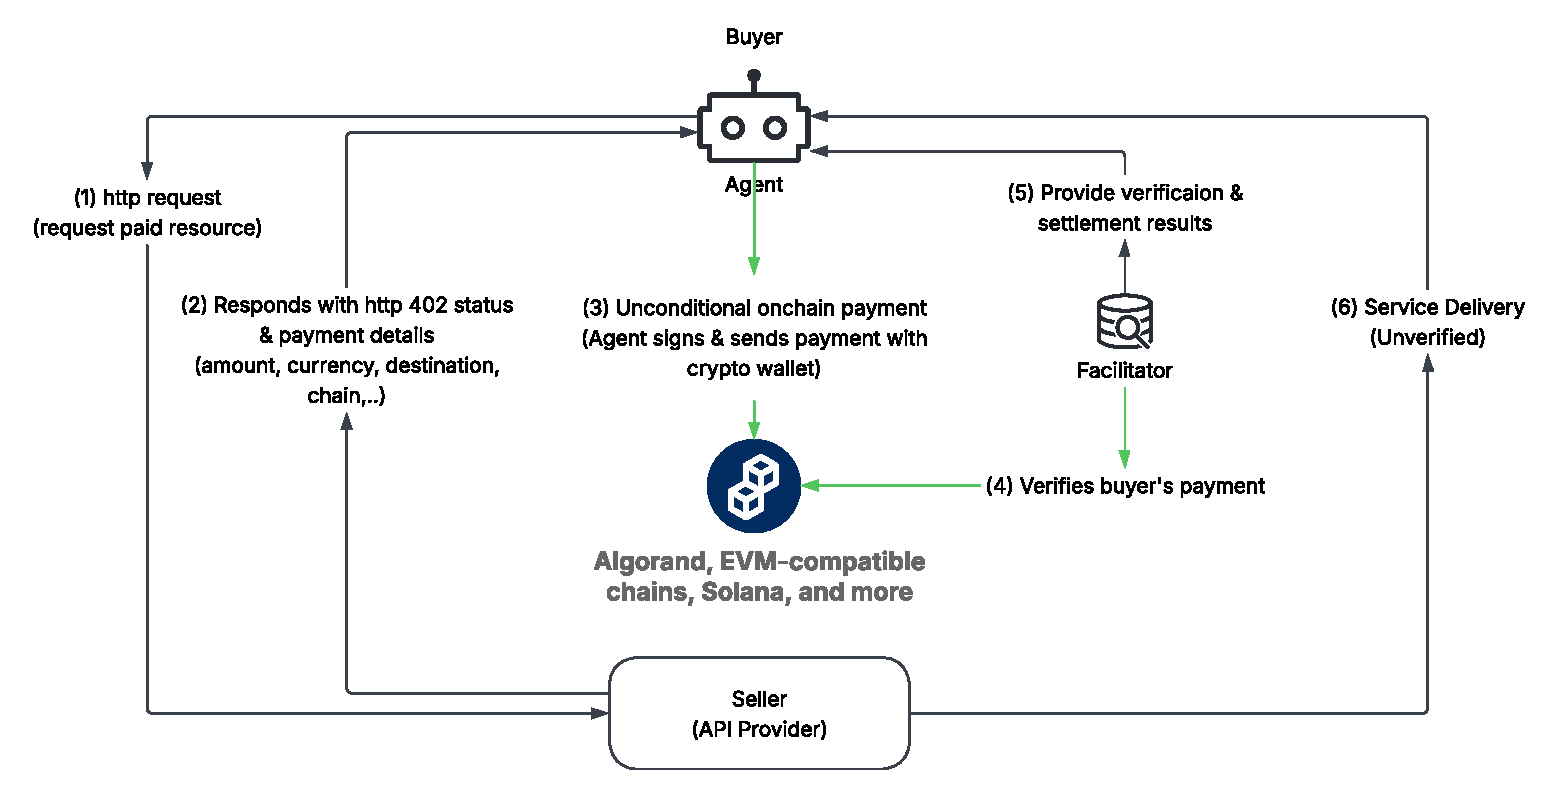
\includegraphics[width=\columnwidth]{Fig1.pdf}
\caption{The standard x402 authorization and escrow flow. The architecture exposes a structural gap where service delivery remains unverified and decoupled from settlement finality (green: on-chain, black: off-chain).}
\label{fig:x402_standard}
\end{figure}
% ============================================================
\section{Background and related work}
% ============================================================

\subsection{HTTP payment and service evidence}

The x402 offer/receipt extension signs payment terms and interaction
records. The x402r auth-capture scheme additionally allows authorization
before resource delivery and later capture or return of funds
\citep{x402receipt,x402r}. T-REX specializes the decision rule through a
committed predicate and registered attestations. It is an HTTP-oriented
settlement design, not a claim of conformance to every x402 scheme or
SDK. Wire-level interoperability requires a separately specified adapter.

The analysis by \citet{li2026five} identifies revert-grant, settlement
preemption, replay/idempotency, header/proxy confusion, and
server-selection attacks. These have different causes. Session binding
and terminal-state checks address particular settlement-layer failure
modes, but do not repair HTTP caching, discovery manipulation, or all
facilitator vulnerabilities. We therefore make no claim that T-REX
eliminates all attacks reported against x402.

A402 studies payment--execution binding using atomic service channels
and trusted execution mechanisms \citep{a402}. RC-S-P formalizes recurring
payment for verifiable services \citep{rcsp}. Their trust assumptions and
service-verification mechanisms differ from a consortium that evaluates
syntactic conditions. An HTLC instead conditions transfer on a preimage
and a deadline; a preimage may be meaningful in an enclosing protocol,
but an HTLC alone does not evaluate the JSON predicates considered here.
These differences motivate capability-aware comparison rather than a
claim that the alternatives lack conditional settlement.

\subsection{Shared evidence and accounting}

Triple-entry accounting motivates a shared, verifiable record connecting
counterparties' records \citep{grigg2024,cai2021}. Blockchain-based
accounting research distinguishes ledger evidence from broader assurance
and reporting responsibilities \citep{dai2017}. T-REX uses ``third entry''
in this evidence-oriented sense: a shared record anchors a settlement
event. It neither replaces double-entry bookkeeping nor determines
whether revenue should be recognized.

\subsection{AVM execution and fees}

Algorand provides an execution environment with atomic transaction
groups and budgeted application calls. Consensus finality and the time a
client observes confirmation are distinct quantities \citep{gilad2017}.
For the evaluated TEAL v11 configuration, each outer application call
contributes 700 cost units to the pooled application budget. Both
\texttt{ed25519verify} and \texttt{ed25519verify\_bare} cost 1,900 units,
but verify different signed message formats \citep{avmopcodes}.
OpUp-style calls obtain additional execution budget using existing
platform facilities; T-REX does not introduce this mechanism
\citep{opup}. Execution units, transaction fees, escrow principal, and
minimum-balance requirements must be accounted for separately.

% ============================================================
\section{System and threat model}
% ============================================================

\subsection{Participants and boundaries}

The participants are a buyer $B$, a seller $S$, three registered
attesters $A_1,A_2,A_3$, a relayer $R$, and an Algorand application.
The buyer authorizes a payment and funds escrow. The seller supplies a
response and signs its commitment. Attesters evaluate the agreed
predicate over the selected response. A relayer submits a terminal call
and receives a funded bounty when that call succeeds.

The attester set is permissioned. Distinct keys do not establish
organizational, infrastructure, or data-source independence. The
prototype's session-scoped provenance policies are an operational trust
boundary, not a cryptographic proof of an authentic TLS transcript.
Cryptographic provenance mechanisms such as DECO may support a stronger
future evidence path, but do not by themselves establish semantic
service quality \citep{deco}.

An adversary may control a buyer or seller, manipulate network delivery,
operate relayer identities, and compromise at most one attester. Safety
does not require timely delivery. Liveness additionally requires the
availability assumptions stated below. Attacks on endpoint selection,
response confidentiality, application governance, and the correctness of
an external AI model are outside the demonstrated protection scope.

\subsection{Assumptions}

\begin{enumerate}
\item[\textbf{A1.}] Ed25519 signatures are unforgeable under the adopted
key-management model, the commitment hashes resist collisions, and the
encoding is unambiguous \citep{rfc8032,fips180}.

\item[\textbf{A2.}] The ledger preserves atomic execution and finality.
Eventual inclusion of valid transactions is assumed only when deriving
liveness; no fixed pre-stabilization inclusion bound is assumed.

\item[\textbf{A3.}] At most one registered attester is Byzantine.
Honest attesters use the same evaluator and agreed response-selection
policy. For a session, they evaluate one common response commitment and
do not sign inconsistent evidence. This common-input condition is an
additional assumption, not a consequence of the threshold alone.

\item[\textbf{A4.}] The relevant contract policy remains fixed: stored
session terms, the attester set, bounty, and terminal routing cannot be
changed during a session. Updates, deletion, emergency controls, or
administrative withdrawals must not invalidate these conditions.

\item[\textbf{A5.}] For liveness, at least one funded submitter observes
the session, can construct a valid transaction, and eventually submits
it. If submission depends on relayer profit, its expected reward must
cover fees, competing-submission risk, and opportunity cost. Attesters
must also be available for an attested transition.
\end{enumerate}

Two quorums of size two can intersect only in a Byzantine attester.
Thus, a 2-of-3 rule is not by itself a Byzantine consensus protocol.
Under A3, each accepted quorum contains an honest signature over the
agreed input. Without common input, blockchain ordering still prevents
two payouts, but does not make the first accepted outcome objectively
correct.

% ============================================================
\section{Protocol specification}
\label{sec:protocol}
% ============================================================
\begin{figure}[htbp]
\centering
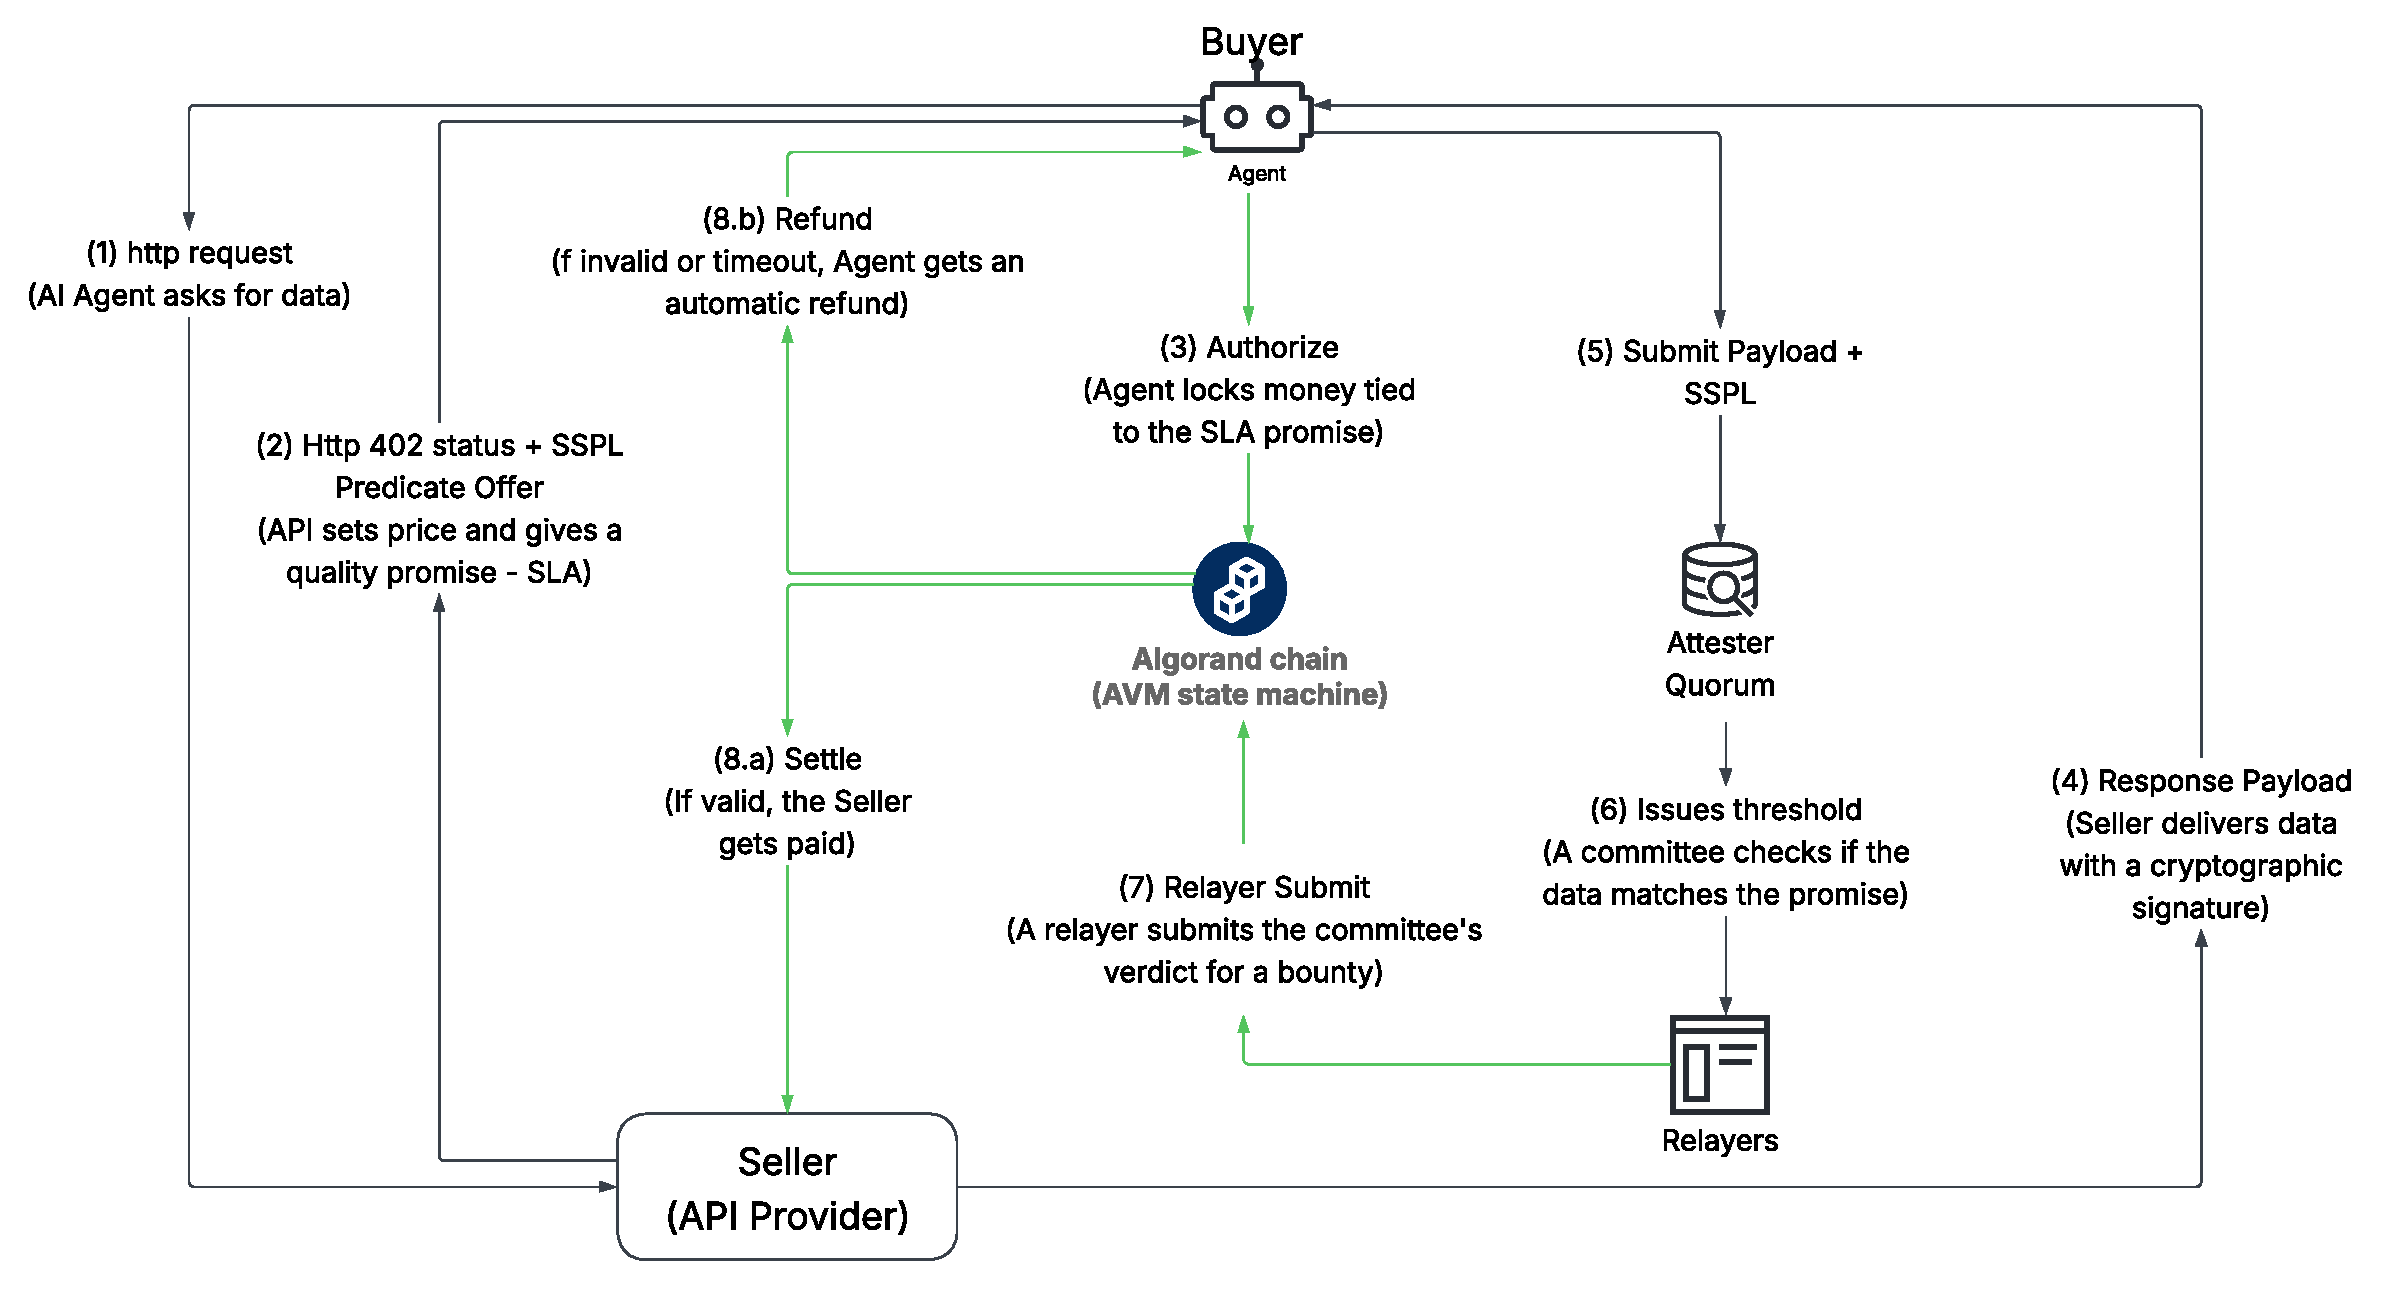
\includegraphics[width=\columnwidth]{Fig2.pdf}
\caption{The T-REX architecture for predicate-conditioned settlement. The protocol decouples the facilitator role via an off-chain Attester Quorum and an economically rational Relayer.}
\label{fig:trex_architecture}
\end{figure}
As illustrated in Fig.~\ref{fig:trex_architecture}, this section defines the abstract protocol and its required checks.
It is not a line-by-line description of every historical executable.
Correspondence to particular deployments is limited to the evidence
identified in Section~\ref{sec:evaluation}.

\subsection{Session identity and committed objects}

Let $g$ be the network genesis hash, $\alpha$ the application ID, and
$n$ a buyer-selected 64-bit nonce. The global session identity is
$u=(g,\alpha,B,n)$. Within one fixed application and network it is
abbreviated to $(B,n)$. The audit identifier $id$ is a buyer-generated
sequence identifier, not an on-chain uniqueness constraint. Nonce reuse
is rejected within this identity namespace.

Let $Q$ be an agreed JSON representation of the HTTP request, $P$ its
predicate, and $J$ the selected JSON response. Define

\begin{equation}
 H_q=\Hash(\JCS(Q)),\quad
 H_c=\Hash(\JCS(P)),\quad
 H_p=\Hash(\JCS(J)).
\end{equation}

JCS supplies canonical JSON serialization \citep{rfc8785}; it does not
define HTTP equivalence. An integration profile must specify the request
method, origin, path, query representation, relevant headers, body
commitment, and response-selection policy. Different profiles must not
be silently treated as equivalent. Duplicate JSON keys and values
outside the supported canonicalization profile are rejected before
commitment.

The stored authorization record is

\begin{equation}
\begin{split}
 C_u=\langle &g,\alpha,B,S,id,n,H_q,H_c,\mathrm{assetId},\\
             &a_{\mathrm{pay}},a_{\mathrm{bounty}},r_{\mathrm{dead}}
             \rangle .
\end{split}
\end{equation}

The payment uses an Algorand asset; the reported bounty uses ALGO.
Amounts are integers in the corresponding smallest units. They are not
added across assets. Network fees and storage funding are separate from
the escrow principal and bounty.

\subsection{SSPL grammar and evaluation}

\begin{definition}[Syntactic predicate grammar]
An SSPL predicate is generated by

\begin{align*}
P ::= {}&\texttt{Compare}(\mathit{path},\mathit{op},\mathit{lit})\\
       &\mid\texttt{And}(P,P)\mid\texttt{Or}(P,P)\mid\texttt{Not}(P),
\end{align*}

where $\mathit{path}$ is an RFC 6901 JSON Pointer \citep{rfc6901},
$\mathit{op}\in\{=,\ne,<,\le,>,\ge\}$, and literals belong to an
agreed scalar type profile. The profile must define numeric precision,
type compatibility, and supported operator/type pairs identically for
all attesters. There is no implicit string-to-number or Boolean-to-number
coercion. Unsupported or structurally invalid comparisons yield $\bot$.
\end{definition}

The evaluation domain is $\{\PASS,\FAIL,\bot\}$. A missing path,
out-of-range array index, or incompatible operand yields $\bot$.
Strong Kleene conjunction and disjunction are shown in
Table~\ref{tab:kleene}. Negation maps $\PASS$ to $\FAIL$, $\FAIL$ to
$\PASS$, and $\bot$ to $\bot$.

\begin{table}[htbp]
\centering
\small
\caption{Strong Kleene binary connectives.}
\label{tab:kleene}
\begin{tabular}{cccc}
\toprule
$x$ & $y$ & $x\land y$ & $x\lor y$\\
\midrule
$\PASS$ & $\PASS$ & $\PASS$ & $\PASS$\\
$\PASS$ & $\FAIL$ & $\FAIL$ & $\PASS$\\
$\PASS$ & $\bot$ & $\bot$ & $\PASS$\\
$\FAIL$ & $\PASS$ & $\FAIL$ & $\PASS$\\
$\FAIL$ & $\FAIL$ & $\FAIL$ & $\FAIL$\\
$\FAIL$ & $\bot$ & $\FAIL$ & $\bot$\\
$\bot$ & $\PASS$ & $\bot$ & $\PASS$\\
$\bot$ & $\FAIL$ & $\FAIL$ & $\bot$\\
$\bot$ & $\bot$ & $\bot$ & $\bot$\\
\bottomrule
\end{tabular}
\end{table}

The signed verdict is $v=\psi(\Eval(P,J))$, where

\begin{equation}
\psi(x)=
\begin{cases}
\PASS,&x=\PASS,\\
\FAIL,&x\in\{\FAIL,\bot\}.
\end{cases}
\end{equation}

This is fail-closed at the root, not a rule that every malformed branch
forces rejection. In particular, $\PASS\lor\bot=\PASS$ and
$\neg(\FAIL\land\bot)=\PASS$. Missing data under a direct negation
remain indeterminate, but errors can be masked by other operands.
Applications requiring every referenced field to be present need a
separate structural-validity condition. SSPL does not establish factual
accuracy, usefulness, or delivery to the buyer.

\subsection{Signature domains and byte encoding}

The revised message domains are

\begin{align}
M_B=\enc\bigl(&\texttt{T-REX-BUY},\alpha,g,B,id,H_q,H_c,
               a_{\mathrm{pay}},\nonumber\\
             &\mathrm{assetId},S,r_{\mathrm{dead}},n\bigr),\\
M_S=\enc\bigl(&\texttt{T-REX-SELL},\alpha,g,B,id,H_q,H_c,
               H_p,r_{\mathrm{dead}},n\bigr),\\
M_A(v)=\enc\bigl(&\texttt{T-REX-ATT},\alpha,g,B,id,H_q,H_c,
               H_p,v,r_{\mathrm{dead}},n\bigr).
\end{align}

Domain tags are literal ASCII bytes without terminators. Integers use
unsigned 64-bit big-endian encoding; addresses, genesis hashes, and
commitment hashes occupy 32 bytes each. The verdict is one byte, with
zero denoting FAIL and one denoting PASS. The attestation message is
therefore 202 bytes. The seller and buyer messages occupy 202 and 217
bytes, respectively. Unsupported widths or values are rejected rather
than truncated. This layout is a specification requirement; interoperability
also requires matching test vectors in the implementation.

Each signature is verified against the appropriate registered key.
The contract reconstructs $g$ and $\alpha$ from its execution context
or immutable deployment state and compares session fields with $C_u$;
accepting caller-selected domains would defeat the binding. Under A1,
signatures for different encoded contexts are not interchangeable.
The guarantee remains conditional on these checks and key security.

The bounty is omitted from $M_B$ only under A4: it is an immutable
application parameter, and authorization checks that the corresponding
bounty is funded. A deployment allowing the bounty or routing policy to
change must introduce a new signed format that explicitly commits those
terms. The seller and attester messages rely on the unique stored
authorization for the payment amount and asset; they are not standalone
authorizations to choose new payment terms.

T-REX's revised domain uses \texttt{ed25519verify\_bare} for direct
verification of these bytes. The other AVM opcode verifies

\[
\texttt{ProgData}\,\|\,\texttt{program\_hash}\,\|\,\texttt{data}
\]

\citep{avmopcodes}. That prefix is an additional domain-separation
mechanism, not a flaw. The bare variant is chosen to match the explicitly
specified off-chain signing format.

\subsection{Threshold acceptance and response selection}

A PASS certificate consists of at least two valid signatures by
\emph{distinct registered attesters} over the same $M_A(\PASS)$.
A FAIL certificate is defined analogously. Duplicate signatures or
repeated signer indices do not increase the count. Insufficient,
invalid, or internally conflicting submissions are rejected.
The attestation threshold is implemented using separate Ed25519
signatures, not an aggregated threshold-signature primitive.

Certificate validation cannot detect all conflicting certificates held
elsewhere. Correctness therefore also relies on A3 and the provenance
policy. In particular, a caller must not be allowed to choose an
unrelated malformed response merely to obtain an early FAIL refund.
Operational tokens must bind the selected response to the intended
session; their adequacy is not established by the on-chain signature
checks alone.

\subsection{Marker lifecycle and transition guards}

For a fixed application, marker keys are

\begin{align}
k_a(B,n)&=\operatorname{SHA512/256}
 (\texttt{T-REX-ACTIVE-NONCE}\|B\|\enc(n)),\\
k_s(B,n)&=\operatorname{SHA512/256}
 (\texttt{T-REX-SPENT}\|\enc(\alpha)\|B\|\enc(n)).
\end{align}

Boxes are scoped to their application. Hashing here provides compact,
domain-separated names; it is not an additional claim about solving a
length-extension attack. The abstract states are Idle, Authorized, Released, and Refunded, as depicted in Fig.~\ref{fig:state_machine}. Table~\ref{tab:transitions} specifies the transition guards.

\begin{figure*}[htbp]
\centering
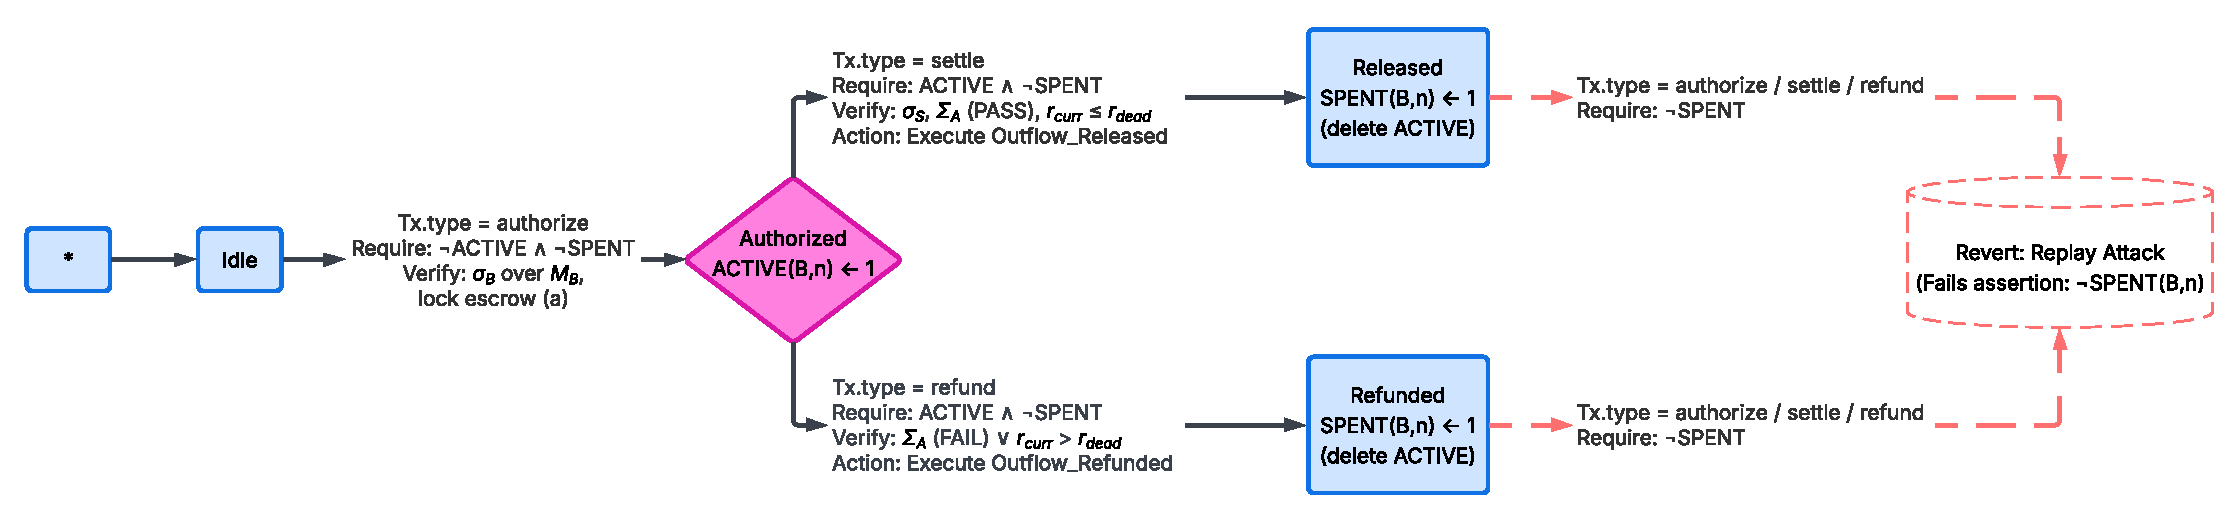
\includegraphics[width=0.85\textwidth]{Fig3.png}
\caption{DFA state transitions and anti-replay marker lifecycle. The \texttt{ACTIVE} marker is ephemeral, while the \texttt{SPENT} marker is persistent, guaranteeing terminal finality without relying on signature consumption.}
\label{fig:state_machine}
\end{figure*}

\begin{table}[htbp]
\centering
\small
\caption{Abstract transition requirements. A failed guard leaves the
session and its asset transfers unchanged.}
\label{tab:transitions}
\begin{tabularx}{\linewidth}{@{}p{0.16\linewidth}YY@{}}
\toprule
Operation & Required checks & Atomic effect\\
\midrule

Authorize &
Neither marker exists; buyer signature valid; terms valid;
payment and bounty deposits match $C_u$; storage funded. &
Store $C_u$, set Authorized, create ACTIVE.\\

Settle &
ACTIVE exists; SPENT absent; stored terms match; seller signature
valid; PASS certificate valid; $r\le r_{\mathrm{dead}}$. &
Pay seller and relayer; create SPENT; delete ACTIVE and releasable
session storage; set Released.\\

Attested refund &
ACTIVE exists; SPENT absent; stored terms match;
FAIL certificate valid. &
Return payment to buyer and pay relayer; create SPENT; delete ACTIVE
and releasable session storage; set Refunded.\\

Timeout refund &
ACTIVE exists; SPENT absent;
$r>r_{\mathrm{dead}}$. &
Same refund routing; no seller or attester signature required.\\

\bottomrule
\end{tabularx}
\end{table}

Authorization must validate transfer type, asset, amount, recipient,
sender authorization, and any close or rekey fields relevant to the
group. Terminal transfers use stored destinations and amounts, not
unchecked arguments. Storage funding and fees must not consume escrow
reserved for another session. These are required enforcement conditions
of the abstract model, not additional tests claimed in this paper.

The current evaluation round determines deadline eligibility. A late
\texttt{settle} call reverts; it does not automatically invoke refund.
A separate valid refund transaction must be submitted. Both attested
refund and timeout lead to the same terminal state, with the first
valid committed transition deciding the session outcome.

\subsection{Routing and receipt structure}

The release and refund routes are

\begin{align}
\mathrm{Release}:&\quad a_{\mathrm{pay}}\rightarrow S,
                       \quad a_{\mathrm{bounty}}\rightarrow R,\\
\mathrm{Refund}:&\quad a_{\mathrm{pay}}\rightarrow B,
                       \quad a_{\mathrm{bounty}}\rightarrow R.
\end{align}

For each asset $k$, escrow accounting requires

\begin{equation}
 D_u^{(k)}=L_u^{(k)}+O_u^{(k)},
\end{equation}

where $D$, $L$, and $O$ denote funded escrow, remaining liability, and
cumulative terminal outflow. Storage balances and network fees are
accounted for outside this equality. A relayer address different from
$B$ or $S$ does not establish a different economic owner and is not an
anti-Sybil guarantee.

A receipt is a tagged record

\begin{equation}
\mathcal R_u=\langle C_u,z,H_p,\sigma_B,\sigma_S,\Sigma_A,
                         \pi_{\mathrm{chain}}\rangle,
\end{equation}

where $z$ is release, attested refund, or timeout refund. Fields not
required for a branch are explicitly absent: a timeout does not require
$H_p$, $\sigma_S$, or $\Sigma_A$, and attested refund does not require
$\sigma_S$. Chain evidence includes network, application, authorization
and terminal transaction identifiers, confirmed rounds, and available
event and transfer records. An indexer response is a retrieval mechanism;
independent verification requires a trusted node or appropriate ledger
proofs, not merely an API response labeled as a proof.

% ============================================================
\section{Safety and conditional liveness}
\label{sec:safety}
% ============================================================

The following arguments concern the abstract transitions above. They
are not a mechanized refinement proof for PyTeal or deployed bytecode.

\begin{proposition}[Terminal uniqueness and replay resistance]
Under atomic execution and permanent SPENT retention, each session
identity has at most one successful terminal transition and cannot be
reauthorized after that transition.
\end{proposition}

\begin{proof}
Initially both markers are absent. Authorization requires their absence
and creates ACTIVE. Every terminal transition requires ACTIVE and the
absence of SPENT, then atomically creates SPENT and removes ACTIVE.
No transition in the model removes SPENT. Consequently a second terminal
transition and a later authorization with the same identity both fail
their guards. Concurrent transactions are serialized by ledger execution;
only the first valid transition can satisfy the preconditions.
\end{proof}

\begin{proposition}[Authorization, binding, and conservation]
Assuming the checks in Table~\ref{tab:transitions}, a release has a prior
funded authorization, valid seller evidence, and a valid PASS
certificate for the stored session. Each asset's terminal outflow is
bounded by that session's funded escrow, and the bounty is paid at most
once.
\end{proposition}

\begin{proof}
Only authorization creates an active session and records its funded
terms. A release requires that state and validates evidence against its
commitments. The only payout operations use the specified routing
amounts. Terminal uniqueness prevents another outflow for the same
identity. Conservation follows separately for the payment asset and
ALGO bounty, provided storage and fees do not draw on their reserved
balances. These premises are essential implementation obligations.
\end{proof}

Binding proves agreement about committed bytes. Under A1 and A3, an
accepted certificate also contains an honest evaluation of the agreed
input. Without provenance and common input, it does not prove delivery
or objective service correctness. A timeout refund likewise proves that
the deadline condition was met, not that the seller necessarily failed
to perform; delayed evidence can cause refund after actual delivery.

\subsection{Termination conditions}

For an attested release before the deadline, the complete evidence,
including the seller signature, must be available early enough for
observation, construction, submission, and inclusion. A sufficient
post-stabilization condition is

\begin{equation}
r_e+\delta_{\mathrm{observe}}+\delta_{\mathrm{build}}
   +\delta_{\mathrm{include}}\le r_{\mathrm{dead}},
\end{equation}

where all quantities are expressed in rounds and $r_e$ is the round at
which the submitter can access complete evidence. Partial synchrony
alone does not supply numerical values for these bounds.

After the deadline, an active session can terminate by timeout if a
submitter can fund and submit the transaction and the ledger eventually
includes it. Contract pause policies, missing resources, insufficient
minimum balance, or unavailable submitters can defeat this premise.
We claim conditional eventual termination, not refund within a fixed
number of rounds under all adversarial schedules. Relayer rationality
is an economic assumption; a positive nominal bounty is not a proof
that some relayer will act.

% ============================================================
\section{AVM budget and fee accounting}
\label{sec:budget}
% ============================================================

\subsection{Verification decomposition}

Buyer authorization is checked before escrow becomes active. A normal
terminal release then requires the seller signature and two attester
signatures; attested refund requires two attester signatures. The
corresponding cryptographic costs are $3\times1,900=5,700$ and
$2\times1,900=3,800$ units. This lifecycle decomposition removes one
signature verification from the terminal path. SSPL evaluation itself
remains off-chain; its restricted grammar supports deterministic
evaluation rather than directly reducing the signature opcode cost.

Fig.~\ref{fig:budget_pooling} illustrates the AVM atomic-group budget pooling mechanism. Table~\ref{tab:profile} reproduces the reported TEAL v11 profiling configurations. The exact bytecode identity of those measurements is
not fully pinned in the accompanying aggregate record. They are not
presented as fresh measurements of App 772170811 after all domain changes.

\begin{figure}[htbp]
\centering
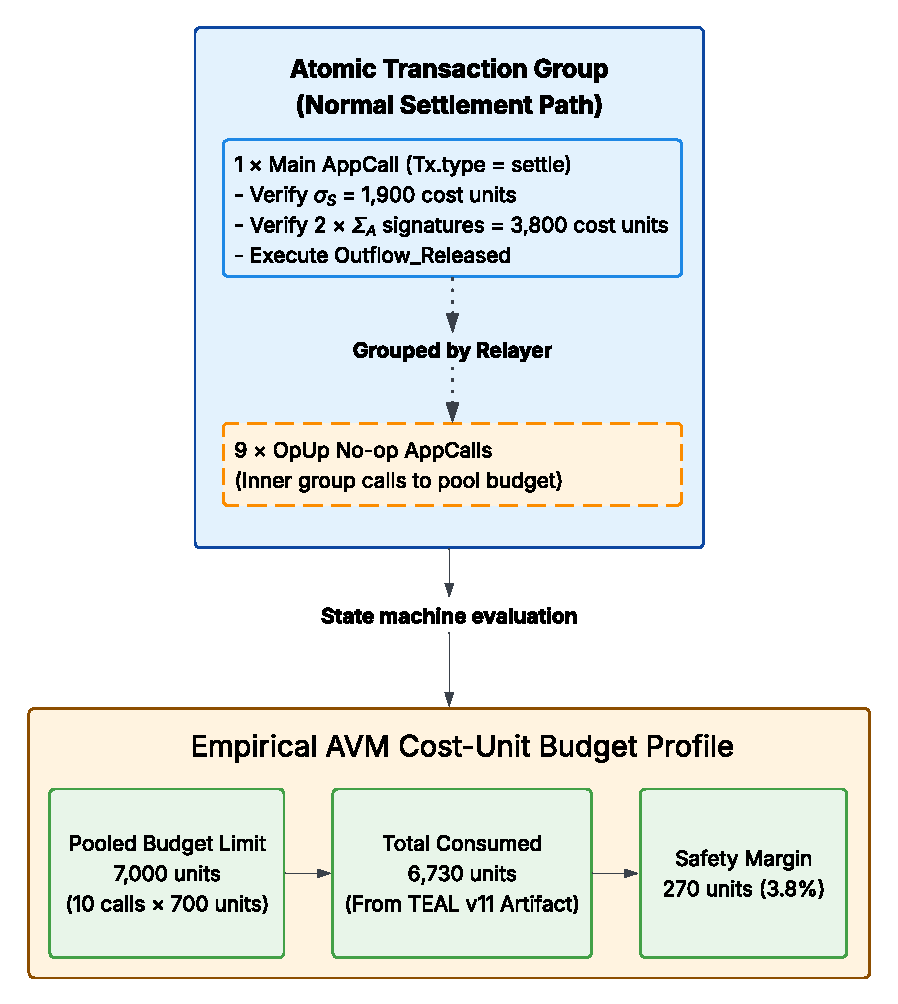
\includegraphics[width=\columnwidth]{Fig4.pdf}
\caption{AVM atomic-group budget pooling. By grouping the main terminal call with OpUp-style dummy calls, the relayer pools sufficient budget to execute multiple cryptographic verifications within a single atomic group.}
\label{fig:budget_pooling}
\end{figure}

\begin{table}[htbp]
\centering
\small
\caption{Reported profiling configurations; budgets use outer AppCalls.
These configurations are distinct from the fee deployment below.}
\label{tab:profile}
\begin{tabular}{lrrrrr}
\toprule
Path & AppCalls & Signature cost & Other cost & Total & Budget\\
\midrule
Release & 10 & 5,700 & 1,030 & 6,730 & 7,000\\
Attested refund & 7 & 3,800 & 711 & 4,511 & 4,900\\
\bottomrule
\end{tabular}
\end{table}

The reported headroom is 270 units (3.86\%) and 389 units (7.94\%).
These are margins for those specific configurations, not worst-case
proofs for all inputs or future versions. Any change to message
construction, guards, or group composition requires renewed profiling.

\subsection{Reported deployed group composition}

The updated fee record describes a different normal-session
configuration: six outer transactions in authorization and sixteen
outer AppCalls plus two inner transfers at settlement. At the stated 1,000-\ualgo{} minimum fee, the accounting is summarized in Table~\ref{tab:fees}.

\begin{table}[htbp]
\centering
\small
\caption{Fee accounting for the reported 16-AppCall terminal
configuration. These are normal-session network fees, excluding escrow,
bounty principal, storage funding, and off-chain costs.}
\label{tab:fees}
\begin{tabularx}{\linewidth}{@{}lYrrr@{}}
\toprule
Group & Composition & Outer & Inner & Fee (\ualgo)\\
\midrule

Authorize &
Asset deposit, ALGO bounty deposit, authorize AppCall,
three budget calls &
6 & 0 & 6,000\\

Terminal &
Settle AppCall and fifteen budget calls; seller and
relayer transfers &
16 & 2 & 18,000\\

Session &
Two separate atomic groups &
22 & 2 & 24,000\\

\bottomrule
\end{tabularx}
\end{table}

The main terminal call is assigned 3,000 \ualgo{} and each of its fifteen
companion calls 1,000 \ualgo{}, covering the two inner transactions
through fee pooling \citep{algofees}. Hence

\begin{equation}
F_{\mathrm{session}}=F_{\mathrm{authorize}}+F_{\mathrm{terminal}}
                    =6,000+18,000=24,000\ \ualgo.
\end{equation}

Its terminal budget is 11,200 units, not 7,000. The 3.86\% margin from
Table~\ref{tab:profile} must not be assigned to this larger group.
Nor is 24,000 \ualgo{} a proven global minimum: if the ten-AppCall
terminal configuration remains valid with the same two inner transfers
and six-transaction authorization, fee arithmetic would give
18,000 \ualgo{} per session. That figure is an analytical alternative,
not a measured optimized deployment. Other resource and guard
requirements must be checked before removing calls.

\subsection{Orchestrator correction and persistent storage}

The historical fee audit reports a terminal charge of 128,000
\ualgo{} under an incorrectly configured orchestrator. Reusing a
\texttt{SuggestedParams} object with an aggregate fee assigned as the
flat fee of each transaction can overpay the group. This is a transaction
construction error, not evidence of a defect in the SDK's documented
per-transaction fee semantics \citep{algosdk}. A recalculated fee is not
itself a new transaction measurement; raw transaction records are
required to confirm the corrected deployment charge.

For a 32-byte box key and one-byte SPENT value, the documented box
minimum-balance increment is

\begin{equation}
2,500+400(32+1)=15,700\ \ualgo
\end{equation}

\citep{boxstorage}. One million such markers therefore lock 15,700
ALGO, apart from other account and session requirements. This is locked
capital, not a network fee. Although deleting a box releases its
minimum-balance requirement, deleting SPENT can invalidate replay
resistance. Safe reclamation requires a replacement replay barrier,
such as an enforced epoch boundary or an authenticated membership
structure. Neither mechanism is evaluated here. Refund-path fees are
not inferred from the normal-session deployment table.

% ============================================================
\section{Audit evidence and accounting integration}
\label{sec:audit}
% ============================================================

The receipt provides evidence inputs rather than an accounting decision.
Table~\ref{tab:audit} maps events to possible downstream use. IFRS 15
recognition depends on the reporting entity's contract and
performance-obligation assessment \citep{ifrs15}; a syntactic PASS is
not a substitute for that assessment. REA supplies a vocabulary for
resources, events, and agents \citep{mccarthy1982}.

\begin{table}[htbp]
\centering
\small
\caption{Illustrative evidence mapping; accounting judgments remain
outside the protocol.}
\label{tab:audit}
\begin{tabularx}{\linewidth}{@{}lYY@{}}
\toprule
Event & Verifiable evidence & Residual assessment\\
\midrule

Authorization &
Signed terms, escrow transfer and session identity &
Contract existence, parties, obligations and collectability\\

Release &
Seller commitment, PASS certificate and asset transfers &
Actual performance, transfer of control and recognition timing\\

Attested refund &
FAIL certificate and refund transfer &
Cause of failure and accounting treatment\\

Timeout refund &
Deadline guard and refund transfer &
Whether service was delivered despite delayed settlement\\

\bottomrule
\end{tabularx}
\end{table}

A minimal export schema comprises the following typed fields, as detailed in Listing~\ref{lst:export}. This is
a proposed interoperability schema, not a claim that an ERP integration
has been evaluated.

\begin{lstlisting}[caption={Typed settlement-evidence export.}, label={lst:export}]
networkGenesisHash: bytes32
applicationId: uint64
buyer: address32
seller: address32
nonce: uint64
auditId: uint64
requestHash: bytes32
predicateHash: bytes32
responseHash: bytes32 | absent
outcome: release | attested_refund | timeout_refund
payment: {assetId: uint64, amountBaseUnits: uint64}
bounty: {amountMicroAlgo: uint64, recipient: address32}
authorizationTxId: AlgorandTransactionId
terminalTxId: AlgorandTransactionId
confirmedRound: uint64
attestations: list<{registeredSignerIndex: uint, signature: bytes64}>
legalDocumentHash: bytes32 | absent
\end{lstlisting}

Amounts are exported as integer base units; an application may serialize
uint64 values as decimal strings to avoid JSON consumer precision loss.
A confirmed round is not a wall-clock timestamp. Any accompanying block
timestamp is stored separately. A legal-document hash is meaningful only
if the agreed request or predicate commits it and the document remains
available. A request hash is not automatically the hash of a legal
document. Such a wrapper supplies an evidentiary link, not a guarantee
of enforceability or automatic recognition.

% ============================================================
\section{Experimental evaluation}
\label{sec:evaluation}
% ============================================================

\subsection{Evidence scope and artifact attribution}

To ensure strict scientific integrity, this evaluation explicitly partitions results by application artifact to prevent the pooling of historical development data with final security validations. The complete raw transaction traces, orchestrator scripts, and TEAL bytecodes for the final unified artifact (App 772170811, commit \texttt{f84a769}) and its associated functional and adversarial campaigns are fully reproducible via the provided repository. Historical campaigns (Apps 769248116 to 772156663) are documented as engineering context to trace the evolution of the AVM budget and marker lifecycle designs, as detailed in Table~\ref{tab:artifacts}.

\begin{table}[htbp]
\centering
\small
\caption{Artifact and campaign attribution. Counts are not pooled across
versions. An unresolved identifier is a reproducibility limitation.}
\label{tab:artifacts}
\begin{tabularx}{\linewidth}
{@{}p{0.22\linewidth}p{0.22\linewidth}Y@{}}
\toprule
Application & Revision locator & Reported evaluation\\
\midrule

769248116 &
\texttt{b654e95} &
Pilot 20 and AVM characterization 30;
historical development results.\\

769453473 &
\texttt{41a5006} &
Campaign C: 100; Campaign D: 180;
historical performance results.\\

770373602 &
Exact revision unresolved &
18 delta-validation tests.\\

770852814 &
Exact revision unresolved &
100 functional sessions:
40 releases, 30 attested refunds, 30 timeout refunds.\\

772156663 &
Exact revision unresolved &
Historical 180-attempt adversarial campaign.\\

772170811 &
\texttt{f84a769} &
Ten targeted negative tests explicitly
associated with this later artifact.\\

Unspecified hardened artifact &
Exact attribution unresolved &
Extended 200-attempt summary; overlap with other series is unresolved.\\

\bottomrule
\end{tabularx}
\end{table}

The reported approval-program identifier for App 772170811 is

\begin{quote}
\footnotesize
\url{RRYTW7VQWWP722I74TFQGPVDE6T2HWPQEJXDP5CGFAXG2UGSJJ62P3OOBM}.
\end{quote}

The source summary abbreviates its clear-program identifier; no full
value is inferred here. A complete reproducibility manifest must also
record the full commit, compiler and SDK versions, network, deployment
transaction, executable bytes, and experiment-to-transaction mapping.
An application ID or program hash alone does not establish these links.

\subsection{Functional results}

The 100-session campaign on App 770852814 reports that all sessions
reached the expected terminal state and that SPENT was retained after
termination. No violation of the monitored terminal-exclusivity or
escrow-conservation checks was reported. These are finite observations,
not proofs over every reachable execution. They are not relabeled as
100 successful sessions on App 772170811. The ten-test record for that
later artifact does not include an equivalent functional-campaign
breakdown.

The earlier 330 sessions are the sum of the 20-session pilot,
30-session characterization, and campaigns C and D. They establish
development history but do not extend the sample size of the
100-session campaign. Similarly, the 18 delta tests and historical
adversarial series are not counted as additional functional sessions.

\subsection{Baseline comparison}

Table~\ref{tab:baseline} retains the reported baseline summary with
30 sessions per listed design. It compares different capabilities;
it is not a performance comparison under equivalent security semantics.

\begin{table}[htbp]
\centering
\small
\caption{Reported baseline summary. Fees are per session; E2E values
are medians. The exact version mapping of these aggregate cells is not
fully resolved.}
\label{tab:baseline}
\begin{tabularx}{\linewidth}{@{}lrrY@{}}
\toprule
Design & Fee (\ualgo) & E2E (s) & Decision mechanism\\
\midrule

Direct payment & 1,000 & 5.28 &
Asset transfer without service escrow\\

HTLC & 4,000 & 11.53 &
Preimage and deadline\\

Naive escrow & 5,000 & 11.20 &
Baseline-specific escrow policy\\

T-REX & 24,000 & 14.93 &
Registered attestations over a predicate-bound response\\

\bottomrule
\end{tabularx}
\end{table}

The listed T-REX fee is 24 times direct payment and six times the HTLC
fee. The 20,000-\ualgo{} difference from HTLC is configuration-specific,
not a universal price of conditional settlement. Attester operations,
storage capital, and service costs are excluded. The four listed cells
account for 120 sessions and are not a complete allocation of the
180-session historical Campaign D. The baseline median of 14.93 seconds
and the functional-campaign mean of 10.11 seconds are different
statistics from separately reported cohorts; they do not establish a
version-to-version speedup.

\subsection{Updated latency decomposition}

The updated timing summary for 40 normal sessions is visualized in Fig.~\ref{fig:latency_decomposition} and detailed in Table~\ref{tab:latency}. Transaction phases are interpreted as
client-observed submission/confirmation intervals. Without detailed
timer boundaries they cannot be separated into pure consensus,
inclusion, RPC, and polling components.

\begin{figure}[htbp]
\centering
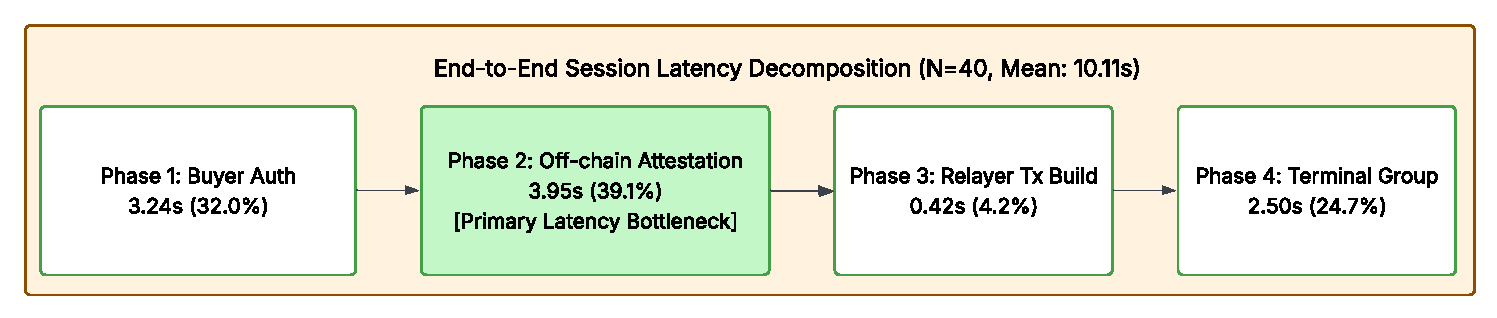
\includegraphics[width=\linewidth]{Fig5.pdf}
\caption{Instrumented end-to-end latency decomposition ($N=40$). Micro-profiling reveals that L1 block finality strictly bounds the system, consuming 95.4\% of the total E2E latency.}
\label{fig:latency_decomposition}
\end{figure}
\begin{table}[htbp]
\centering
\small
\caption{Updated aggregate timing summary for normal sessions
($N=40$). Ranges describe observations, not confidence intervals.}
\label{tab:latency}
\begin{tabularx}{\linewidth}{@{}Yrrr@{}}
\toprule
Phase & Mean (s) & Min--max (s) & Share\\
\midrule

Authorization/confirmation &
4.73 & 4.38--6.95 & 46.8\%\\

Off-chain attestation and relayer &
0.47 & 0.40--0.55 & 4.6\%\\

Terminal submission/confirmation &
4.91 & 4.63--5.06 & 48.6\%\\

Total E2E &
10.11 & 9.64--12.24 & 100\%\\

\bottomrule
\end{tabularx}
\end{table}

At the reported precision, the two transaction phases account for
95.4\% of the total. The earlier decomposition assigned 3.24 seconds
to authorization, 3.95 to attestation, 0.42 to relayer construction, and
2.50 to terminal confirmation, while retaining the same total.
The updated table supersedes that phase allocation; the available
summaries do not identify the instrumentation or data-mapping change
responsible. This is an unresolved measurement-provenance limitation.
Accordingly, we draw only the configuration-specific observation that
the updated summary is dominated by transaction-observation intervals.
It does not demonstrate an immutable L1 latency floor, a mandatory need
for L2 migration, or an on-chain execution bottleneck.

\subsection{Targeted security checks on App 772170811}

\begin{table}[htbp]
\centering
\small
\caption{Reported targeted negative tests on App 772170811,
revision \texttt{f84a769}. All ten attempts were rejected.}
\label{tab:targeted}
\begin{tabularx}{\linewidth}{@{}YrY@{}}
\toprule
Mutation or attempted transition & Count & Reported rejection\\
\midrule

Zero/Mainnet genesis in signed domain &
2 & Signature verification\\

Wrong buyer in attestation domain &
1 & Signature verification\\

Different application ID &
1 & Signature verification\\

Altered deadline &
1 & Signature verification\\

Corrupted seller or attester signature &
2 & Signature verification\\

Altered response commitment &
1 & Signature verification\\

Second settlement after release &
1 & Session box absent\\

Premature timeout &
1 & Deadline assertion\\

\midrule
Total & 10 & No successful negative attempt reported\\
\bottomrule
\end{tabularx}
\end{table}

As detailed in Table~\ref{tab:targeted}, these results support the rejection of the submitted test cases. They do
not establish exhaustive security or probabilistic exploit resistance.
The cross-domain cases require particular care: changing a message
without regenerating its signature tests message integrity, whereas
replaying a correctly signed message from a different context tests the
domain-binding policy. The aggregate table does not fully document that
construction distinction.

The second-settlement case demonstrates rejection after the session box
has been removed. It does not alone establish SPENT retention or
rejection of a subsequent authorization with the original nonce.
Complete regression coverage additionally needs positive controls,
reauthorization after both outcomes, duplicate/unregistered signers,
conflicting certificates, transfer-field mutations, and deadline-boundary
cases. Those additional cases are not claimed as completed on this
artifact merely because historical versions contain related tests.

\subsection{Extended adversarial record}

An additional supplied study table reports 200 negative attempts and
zero successful exploits: 40 reauthorizations after terminal outcomes,
and 20 each for duplicate settlement, concurrent authorization,
payload tampering, bad attester signatures, deadline tampering,
cross-user replay, cross-instance replay, and cross-network replay.
The counts sum to 200. However, that table does not identify a complete
artifact locator or establish whether its first 180 attempts overlap
the earlier campaign. We therefore report it as a separate extended
record, do not add it to the ten targeted tests, and do not attribute
its program counters to App 772170811. Program counters are meaningful
only with the corresponding executable and source map.

\subsection{Distribution fitting and limits of simulation inference}

The updated fit summary, presented in Table~\ref{tab:fits}, uses a two-parameter lognormal model $X=\theta\exp(sZ)$, $Z\sim\mathcal N(0,1)$, with location fixed at zero.
Its expectation is $\theta\exp(s^2/2)$.

\begin{table}[htbp]
\centering
\small
\caption{Reported exploratory lognormal fits and calculated expectations.
Agreement of means is not a goodness-of-fit or tail-validation result.}
\label{tab:fits}
\begin{tabular}{lrrrr}
\toprule
Phase & $s$ & $\theta$ & Model mean (s) & Reported mean (s)\\
\midrule
Authorize & 0.0734 & 4.7142 & 4.7269 & 4.7283\\
Terminal & 0.0170 & 4.9078 & 4.9085 & 4.9085\\
E2E & 0.0375 & 10.0995 & 10.1066 & 10.1069\\
\bottomrule
\end{tabular}
\end{table}

The listed expectations agree with the reported means to approximately
0.03\% or better. This arithmetic check does not validate the full
distribution. A positive location parameter is not inherently invalid;
a fitted support must instead be compatible with the observations.
Fixing the location at zero is a modeling choice, not proof of a
physical latency law.

The timing record and fitted tails warrant caution. For example, the
authorize parameters imply

\begin{equation}
\Pr(X\ge6.95)
=1-\Phi\!\left(\frac{\log(6.95/4.7142)}{0.0734}\right)
\approx6.2\times10^{-8},
\end{equation}

although 6.95 seconds is the reported maximum among 40 observations.
This diagnostic does not constitute an independent hypothesis test on
parameters fitted from those data. It does show why mean agreement
cannot justify claims that timeout-relevant tails are preserved.

The accompanying narrative mentions low asymptotic KS p-values without
providing a complete calibrated test output. They are not dismissed as
harmless consequences of a step-shaped empirical CDF. When parameters
are estimated from the tested observations, an appropriate parametric
bootstrap refits them within each replicate \citep{scipygof}.
Correlated phase delays, clustered confirmations, and endpoint-specific
polling also require examination. No production throughput, validated
timeout probability, or simulation-based security rate is inferred from
these exploratory fits. Earlier synthetic throughput estimates are
excluded from the empirical conclusions.

% ============================================================
\section{Discussion and limitations}
% ============================================================

\subsection{Interpretation of the research questions}

For RQ1, the protocol gives explicit binding and state-transition
requirements; the reported tests exercise only a subset of them. For
RQ2, historical profiling supports feasibility of pooled signature
verification, while the deployment fee record documents a larger group
configuration. For RQ3, safety follows for the stated abstract model and
liveness is conditional on evidence availability and transaction
inclusion. For RQ4, the receipt and export fields support an evidence
mapping, without demonstrating accounting recognition or ERP adoption.

The practical contribution is a reproducible specification target and
a bounded account of prototype evidence. The restricted predicate
language, ordinary signatures, and OpUp mechanism are not claimed as
new cryptographic primitives. Differences from other payment systems
must be interpreted together with their trust and verification models.

\subsection{Threats to validity}

Internal validity is limited by incomplete experiment-to-bytecode
mapping, unresolved changes to phase timing, and the distinction
between corrected fee arithmetic and confirmed corrected transactions.
Construct validity is limited because a client confirmation timer is
not a direct consensus measurement and an attester verdict is not
objective service correctness. Statistical validity is limited by the
small normal-session sample, unavailable raw traces for independent
reanalysis, and unvalidated tail models. External validity is limited
by Testnet execution and the permissioned gateway setting.

The protocol does not guarantee symmetric fair exchange for an
irreversible service: a buyer may receive a response before settlement,
and a timeout may return payment after delivery. Attester collusion,
common-source failures, compromised provenance, or governance changes
can invalidate stronger interpretations of the guarantee. Economic
compensation alone is not demonstrated resistance to bribery.

A per-session network fee of 0.024 ALGO has no universal dollar-based
viability threshold. Its significance depends on exchange rate,
service value, attester operating costs, storage capital, and transaction
volume. Claims about sub-cent viability or mandatory batching require
those assumptions. Similarly, an upgrade proxy is not a necessary
consequence of a tight opcode margin and would introduce additional
governance and replay obligations.

\subsection{Further validation}

The next validation step is one pinned executable with positive and
negative tests, per-transaction fees, per-session timer boundaries, and
complete compiler and source maps. Further work includes independently
specified response provenance, deterministic evaluator conformance
vectors, safe replay-state reclamation, and a mechanized relationship
between the transition system and executable checks. TLS provenance
and semantic quality assessment remain separate research problems.

% ============================================================
\section{Conclusion}
% ============================================================

T-REX specifies a threshold-attested settlement workflow that binds
buyer authorization, an HTTP request commitment, a syntactic predicate,
and response evidence to a unique release or refund transition.
Its safety arguments depend on explicit encoding, storage, routing,
and attestation assumptions. The blockchain enforces the decision
procedure; it does not independently establish response provenance or
semantic service quality.

By explicitly bounding its claims to syntactic settlement and 
configuration-specific AVM accounting, T-REX provides a reproducible, 
ledger-verified foundation for future HTTP-native agentic commerce, 
establishing a rigorous baseline for subsequent research in 
cryptographic provenance and L2 throughput.

% ============================================================
\appendix
\section{Abstract proof obligations and reproducibility boundaries}
% ============================================================

Let $T_u$ count successful terminal transitions and $A_u$ record whether
authorization has ever occurred. Initially $T_u=0$, $A_u=0$, and both
markers are absent. Authorization sets $A_u=1$ and ACTIVE. A terminal
transition increments $T_u$, removes ACTIVE, and sets SPENT.
Induction over the specified transitions gives

\begin{align}
&T_u\in\{0,1\},\\
&T_u=1\ \Longrightarrow\ \Spent(u)\land\neg\Active(u),\\
&T_u=1\ \Longrightarrow\ A_u=1,\\
&\Spent(u)\ \Longrightarrow\ \neg\mathrm{AuthorizeAllowed}(u).
\end{align}

The historical statement ``Released implies Authorized'' must be read
as prior authorization, not simultaneous occupancy of two DFA states.
These invariants assume SPENT is never deleted and contract policy does
not bypass the transition guards.

The earlier TLA+ listing was a partial sketch. No complete model,
configuration, invariant definitions, state counts, or TLC output is
available in the records used here to substantiate a model-checking
result. This revision therefore presents the explicit abstract argument
above and makes no claim that TLC or Coq has verified the executable.
An implementation refinement proof would additionally need to relate
storage encoding, transaction-group checks, signature domains, and
asset transfers to these abstract variables.

For reproducibility, each published numerical row should resolve to a
manifest entry containing network genesis, application and deployment
identifiers, full source revision, executable hashes, toolchain versions,
group-construction parameters, scenario, raw record location, and the
analysis command. Reported aggregate tables without those links are
identified as such in Section~\ref{sec:evaluation}; unspecified values
are not reconstructed from program-counter coincidences or filenames.

% ============================================================
\section*{Data and code availability}
% ============================================================

The core protocol specification, the final hardened smart contract 
artifact (App ID 772170811), the 202-byte message domain generators, 
and the raw CSV traces for the 100-session functional campaign and the 10 targeted adversarial tests are openly archived at \url{https://github.com/leminhtuan/TREX}. 
While the exact intermediate orchestrator states of historical 
development campaigns are provided as raw ledger dumps rather than fully containerized pipelines, the final security boundaries, fee accounting, and latency distributions reported in this manuscript can be independently verified and reproduced using the provided Testnet transaction IDs and Python evaluation scripts.

% ============================================================
\section*{AI assistance disclosure}
% ============================================================

Generative AI assisted with manuscript restructuring, language editing,
LaTeX drafting, and consistency checks. This assistance did not execute
the reported blockchain campaigns or independently establish their
results. Responsibility for the data, implementation, references, and
scientific conclusions remains with the author.

% ============================================================
\section*{Acknowledgments}
% ============================================================

This work was supported by Hanoi Open University under Project
MHN2026-CT01-03.

% ============================================================
\section*{Competing Interests}
% ============================================================
The author declares no competing interests.

% ============================================================
\section*{Author Contributions}
% ============================================================
Minh Tuan Le conceived and designed the research, performed the 
smart contract implementations and Testnet experiments, analyzed 
the data, and wrote the manuscript.

\begin{thebibliography}{99}
% ============================================================

\bibitem[Fielding et al.(2022)]{http9110}
Fielding, R., Nottingham, M., and Reschke, J. (2022).
HTTP Semantics. RFC 9110.
\url{https://doi.org/10.17487/RFC9110}.

\bibitem[x402(2026a)]{x402docs}
x402 (2026a). x402 documentation.
\url{https://docs.x402.org/}.
Accessed 21 September 2026.

\bibitem[x402(2026b)]{x402receipt}
x402 (2026b). Signed Offers \& Receipts.
\url{https://docs.x402.org/extensions/offer-receipt}.
Accessed 21 September 2026.

\bibitem[x402r(2026)]{x402r}
x402r (2026). auth-capture Scheme.
\url{https://docs.x402r.org/x402-integration/auth-capture}.
Accessed 21 September 2026.

\bibitem[Asokan et al.(1998)]{asokan1998}
Asokan, N., Shoup, V., and Waidner, M. (1998).
Optimistic fair exchange of digital signatures.
In \emph{EUROCRYPT '98}, pp. 591--606.
\url{https://doi.org/10.1007/BFb0054156}.

\bibitem[Abadi et al.(2023)]{rcsp}
Abadi, A., Murdoch, S. J., and Zacharias, T. (2023).
Recurring Contingent Service Payment.
In \emph{IEEE European Symposium on Security and Privacy},
pp. 724--756.
\url{https://doi.org/10.1109/EuroSP57164.2023.00049}.

\bibitem[Li et al.(2026a)]{li2026five}
Li, Z., Wang, Q., and Wang, Z. (2026a).
Five Attacks on x402 Agentic Payment Protocol.
arXiv preprint 2605.11781.
\url{https://arxiv.org/abs/2605.11781}.

\bibitem[Li et al.(2026b)]{a402}
Li, Y., Wang, L., Wang, K., Yang, Z., Wang, K., Guan, Z., and Gao, J.
(2026b). A402: Binding Cryptocurrency Payments to Service Execution
for Agentic Commerce.
arXiv preprint 2603.01179.
\url{https://arxiv.org/abs/2603.01179}.

\bibitem[Grigg(2024)]{grigg2024}
Grigg, I. (2024). Triple Entry Accounting.
\emph{Journal of Risk and Financial Management}, 17(2), 76.
\url{https://doi.org/10.3390/jrfm17020076}.

\bibitem[Cai(2021)]{cai2021}
Cai, C. W. (2021).
Triple-entry accounting with blockchain: How far have we come?
\emph{Accounting \& Finance}, 61(1), 71--93.
\url{https://doi.org/10.1111/acfi.12556}.

\bibitem[Dai and Vasarhelyi(2017)]{dai2017}
Dai, J., and Vasarhelyi, M. A. (2017).
Toward Blockchain-Based Accounting and Assurance.
\emph{Journal of Information Systems}, 31(3), 5--21.
\url{https://doi.org/10.2308/isys-51804}.

\bibitem[Gilad et al.(2017)]{gilad2017}
Gilad, Y., Hemo, R., Micali, S., Vlachos, G., and Zeldovich, N. (2017).
Algorand: Scaling Byzantine Agreements for Cryptocurrencies.
In \emph{SOSP '17}, pp. 51--68.
\url{https://doi.org/10.1145/3132747.3132757}.

\bibitem[Algorand(2026a)]{avmopcodes}
Algorand (2026a). AVM Opcodes.
\url{https://dev.algorand.co/reference/algorand-teal/opcodes/}.
Accessed 21 September 2026.

\bibitem[Algorand(2026b)]{opup}
Algorand (2026b). OpUp---PyTeal Documentation.
\url{https://pyteal.readthedocs.io/en/stable/opup.html}.
Accessed 21 September 2026.

\bibitem[Algorand(2026c)]{algofees}
Algorand (2026c). Transaction Fees.
\url{https://dev.algorand.co/concepts/transactions/fees/}.
Accessed 21 September 2026.

\bibitem[Algorand(2026d)]{algosdk}
Algorand (2026d). Python SDK: Transaction and SuggestedParams.
\url{https://py-algorand-sdk.readthedocs.io/en/latest/algosdk/transaction.html}.
Accessed 21 September 2026.

\bibitem[Algorand(2026e)]{boxstorage}
Algorand (2026e). Box Storage.
\url{https://dev.algorand.co/concepts/smart-contracts/storage/box/}.
Accessed 21 September 2026.

\bibitem[Josefsson and Liusvaara(2017)]{rfc8032}
Josefsson, S., and Liusvaara, I. (2017).
Edwards-Curve Digital Signature Algorithm (EdDSA).
RFC 8032.
\url{https://doi.org/10.17487/RFC8032}.

\bibitem[NIST(2015)]{fips180}
National Institute of Standards and Technology (2015).
Secure Hash Standard (SHS). FIPS PUB 180-4.
\url{https://doi.org/10.6028/NIST.FIPS.180-4}.

\bibitem[Rundgren et al.(2020)]{rfc8785}
Rundgren, A., Jordan, B., and Erdtman, S. (2020).
JSON Canonicalization Scheme (JCS). RFC 8785.
\url{https://doi.org/10.17487/RFC8785}.

\bibitem[Bryan et al.(2013)]{rfc6901}
Bryan, P., Zyp, K., and Nottingham, M. (2013).
JavaScript Object Notation (JSON) Pointer. RFC 6901.
\url{https://doi.org/10.17487/RFC6901}.

\bibitem[Zhang et al.(2020)]{deco}
Zhang, F., Maram, D., Malvai, H., Goldfeder, S., and Juels, A. (2020).
DECO: Liberating Web Data Using Decentralized Oracles for TLS.
In \emph{ACM CCS '20}, pp. 1919--1938.
\url{https://doi.org/10.1145/3372297.3417239}.

\bibitem[IFRS Foundation(2026)]{ifrs15}
IFRS Foundation (2026).
IFRS 15 Revenue from Contracts with Customers.
\url{https://www.ifrs.org/issued-standards/list-of-standards/ifrs-15-revenue-from-contracts-with-customers/}.
Accessed 21 September 2026.

\bibitem[McCarthy(1982)]{mccarthy1982}
McCarthy, W. E. (1982).
The REA Accounting Model: A Generalized Framework for Accounting
Systems in a Shared Data Environment.
\emph{The Accounting Review}, 57(3), 554--578.

\bibitem[SciPy(2026)]{scipygof}
SciPy (2026).
\texttt{scipy.stats.goodness\_of\_fit}.
\url{https://docs.scipy.org/doc/scipy/reference/generated/scipy.stats.goodness_of_fit.html}.
Accessed 21 September 2026.

\end{thebibliography}

\end{document}
